At the beginning of the 20$\textsuperscript{th}$ century the world underwent the first quantum revolution. New ideas about wave-particles duality and quantization gave scientists the tools to explain previously observed phenomena such as the periodic table, chemical interactions, and electronic wavefunctions. With a deeper understanding, this new quantum theory drove revolutionary technologies such as electronic semiconductors thus bringing the world into the Information age. Now we are undergoing a second quantum revolution where we are no longer using quantum mechanics to simply explain observed phenomena, we are actively \textit{controlling} quantum mechanics.\cite{Dowling2003} We are using quantum technologies to organize and build complex systems at the atomic level. This extraordinary leap forward has allowed us to create and research new quantum phases of matter and their associated new quasi-particles. Much as before, research into new quantum phases of matter is paramount for driving new technologies forward. For example, research into high-temperature superconductivity may lead us to room-temperature superconductivity, a phenomena which would massively reduce energy dissipation in modern electronics. However, it can be quite difficult to tell whether or not a system is in a new phase, especially if that phase is topological. Furthermore, once the system is in a new phase, robustly measuring the emergent modes requires new techniques and ideas. In this dissertation, we describe the development of new equipment to help build these new quantum tools as well as the novel iron-based topological superconducting system such equipment has allowed us to study.
\section{Scope}
The works presented in this dissertation fall into two main parts: advances in nano-fabrication equipment and topological superconductivity. The first part introduces recent advances in condensed matter physics along with the difficulties associated with fabricating electronic devices to better study these new topics. In particular, we discuss nano-fabrication with materials that are acutely air-sensitive such as GdTe$_{3}$ as well as with materials where the bulk is stable in air but have air-sensitive surfaces such as \ac{FTS}. The latter materials are of particular interest since the emergent modes that are indicative of a topological phase are often found on the surface of the material. The second part dives into the subject topological superconductors and higher order topology. Specifically, we focus on the iron-based superconductor \acl{FTS}, its topological properties, and some exciting new experiments.\par
The rest of this introduction will review pertinent background material. We introduce the notion of emergence and quantum phases of matter with specific applications to superconducting materials. We will leave some subjects of superconductivity, e.g. tunneling into a superconductor from a normal metal, to the appendices where these subjects can get a more in-depth treatment. A brief overview of topology will be given but more focus will be spent on how to treat the notion of topology in superconductivity.
\section{Emergence and Topology}
Emergence can be colloquially summarized as, ``The whole is greater than the sum of its parts." Examples of emergence are all around us, from the biggest of scales where galaxies coalesce into superclusters to the smallest of scales where atoms emerge out of the fundamental excitations of quantum fields. With such a huge subject, it is easy to see why studying emergence is of such importance, i.e., discoveries made about an emergent behavior may have useful applications in other disciplines. While this is exciting, it can also be easy to be sidetracked onto other topics and applications. Thus to keep this work on track we will use the sharper definition provided by Kivelson \& Kivelson:
\begin{quote}
	``An emergent behavior of a physical system is a qualitative property that can only occur in the limit that the number of microscopic constituents tends to infinity."\cite{Kivelson2016}
\end{quote}
Phases of matter are a fantastic example of this definition as the same constituent material can display vastly different properties. Indeed, even small changes to the interactions between these microscopic constituents can lead a ``classic" system (such as metals or insulators) to new phases of matter such as superconductivity and magnetism. Accompanying these phases are often new, useful quasi-particles such as the cooper pair and the magnon from the examples before. Not only do these new quasi-particles have value in real-world applications, they are also a critical method of identifying a new phase. Thus a governing question for the rest of this work is as follows, ``What parameters can we tune to create a brand new phase of matter and what quasi-particles will this new phase produce?"
\par 
Many of electronic phases can be described elegantly through the language of symmetry and symmetry breaking\cite{Noether1918, Landau1937, pathria_beale_2022}. However, starting in 1980 evidence began emerging that not all phases and phenomena could be explained by the use of symmetry alone. The first example of such a phase was the Quantum Hall Effect wherein a two-dimensional electron gas exhibits exactly quantized Hall voltages at large, perpendicular magnetic fields\cite{Klitzing1980}. This phase consists of an insulating bulk with a perfectly ballistic 1-D edge mode around the bulk. Moreover, the phase does not immediately arise when time-reversal symmetry is broken but instead emerges at a finite magnetic field with no additional symmetries being broken. The Hall conductance increases by exact multiples of the quantum of conductance ($e^{2}/h$) by further increasing the magnetic field, indicating more edge modes are emerging\cite{Zhang2005}. It was later shown that these quantized plateaus can be described using a topological invariant $C_{n}$ called the Chern number.\cite{Thouless1982, Kohmoto1985, Avron1983, Niu1985}\par 
This Chern number is one example of a topological invariant arising from what is known as the Berry Phase\cite{Berry1984}. The Berry phase is an additional, gauge-invariant phase factor acquired by a quantum mechanical system when it adiabatically evolves through a cyclical process and may be expressed as\cite{Berry1984, Xiao2010}:
\begin{align}
	\gamma_{n} = i\oint_{C}\bra{n(\textbf{R})}\nabla\ket{n(\textbf{R})}\cdot d\textbf{R}
\end{align}
where $\gamma_{n}$ is the Berry phase, $\ket{n(\textbf{R})}$ is the wave function for an arbitrary parameter $\textbf{R}$, and $C$ is a closed loop in the parameter space. As an aside, this parameter $\textbf{R}$ is commonly either the crystal momentum $k$, or the spatial position, however the general theory describes a closed loop in \textit{any} parameter space, which leads to some interesting topological phenomena\cite{Onoda2002,Gobel2019}. The Chern number arises when integrating this Berry phase of the wavefunction in momentum space and while defining and describing the Chern number in its full glory is fascinating, it is not within the scope of this dissertation as the rest of these works are focused on another topological invariant, the $\mathbb{Z}_{2}$ invariant.\par 
Before we move onto a discussion of the $\mathbb{Z}_{2}$ invariant and topological superconductivity I would like to make a quick note. The 1-D edge modes that arise in the Quantum Hall Effect are a beautiful example of how new phases often come with new quasiparticles. In the next section, we provide an example of another emergent quasi-particle. One that is central to the works presented in this dissertation, the Majorana Zero Mode.
\section{Topological Superconductivity}
The $\mathbb{Z}_{2}$ invariant as applied to 2D electronic systems first arose in 2005 when it was noted that imposing time-reversal symmetry in such systems leads to new topological invariants\cite{Kane2005, Onoda2002, Shuichi_Murakami_2007}. While nonzero Chern numbers cannot be realized with time-reversal invariance, the ``zero" Chern-number class instead can be subdivided into two pieces: ``ordinary" insulators that do not in general have an edge state, and a ``Quantum Spin Hall Effect" where a bulk topological invariant forces an edge state. The topological invariant in this case is not an integer, but rather a two-valued or $\mathbb{Z}_{2}$ invariant. Physically, this idea can be thought of as having two copies of the Quantum Hall Effect, one for spin-up electrons and one for spin-down, with opposite propagation directions. This system remains time-reversal invariant because time-reversal flips both the spin and propagation direction, thus both copies ``transform" into each other under this operation. To understand how this leads to two-valued invariant rather than an integer invariant we need to take a look at how the time-reversal operator $\mathcal{T}$ acts in Fermi (half-integer spin) systems. In 1930, H. A. Kramers showed that the square of the time-reversal operator is connected to a $2\pi$ rotation implying:
\begin{align}
	\mathcal{T}^{2} = (-1)^{2S}
\end{align}
where $S$ is the total spin quantum number of a state\cite{Kramers1930}. Plugging in half-spin shows that Fermion systems pick up a minus sign under two time-reversal operations. An immediate consequence of this is that every eigenstate of a time-reversal-invariant spin-half system is at least two-fold degenerate, also known as ``Kramers pairs". A non-rigorous proof is by showing that a time-reversal invariant perturbation $H'$ cannot mix members of a Kramers pair.
\begin{align}
	\bra{\mathcal{T}\psi}H'\ket{\psi} &= \bra{\mathcal{T}\psi}H'\ket{\mathcal{T}^{2}\psi} \tag*{$\mathcal{T}$ is antiunitary and H' is TRS}\\
	\bra{\mathcal{T}\psi}H'\ket{\mathcal{T}^{2}\psi} &= -\bra{\mathcal{T}\psi}H'\ket{\psi} \tag*{$\mathcal{T}^{2} = -1$}\\
	\therefore \bra{\mathcal{T}\psi}H'\ket{\psi} &= -\bra{\mathcal{T}\psi}H'\ket{\psi} = 0
	\tag*{$x = -x \implies x = 0$}
\end{align}
We can now combine this Kramers pair knowledge with the counter-propagating edge states mentioned above. If there is only a single Kramers pair of edge states then a right-moving excitation can only backscatter into its time-reversal conjugate, which we just showed is forbidden if the perturbation inducing scattering is time-reversal invariant. However, if we have two Kramers pairs of edge modes, then a right-mover can backscatter to the left-mover of the \textit{other} Kramers pair, since it is not its time-reversal conjugate, which will eliminate the two Kramers pairs. Thus a system with an even number of Kramers pairs will pair down to zero Kramers pairs (making a trivial insulator), whereas systems with an odd number of Kramers pairs will wind up with a single, stable Kramers pair (a non-trivial insulator)\cite{Hasan2010}. Thus a topological system with time-reversal invariance will have a two-valued invariant that is either even or odd.\par
For an immediate consequence of this result on Fermionic systems we turn to the toy model of p-wave superconductivity on a 1D wire. We will start with the \ac{BdG} equations of which there is an in-depth derivation of presented in Appendix \ref{app:ARfit}, here we will use the final Hamiltonian from that appendix with some minor alterations. We will be closely following the works of Kitaev and Bernevig \& Hughes\cite{Kitaev2001, bernevig_hughes_2013}.\par 
We begin by describing a 1-D chain of fermions, i.e., at each lattice site $j$ on the chain there is a complex fermion $c_{j}$. For simplicity, we consider these complex fermions to either be spinless or fully spin-polarized due to a source of time-reversal symmetry breaking. Since a momentum-independent s-wave pairing potential is not possible for spinless fermions, we will use a momentum-dependent p-wave potential (in momentum space):
\begin{align}
	H_{\Delta} = \frac{1}{2}\left(\Delta pc_{p}^{\dagger}c_{-p}^{\dagger}+\Delta^{*}pc_{-p}c_{p}\right)
\end{align}
where $c^{\dagger}$ and $c$ are the creation and annihilation operators, $p$ is the momentum, and $\Delta$ is the superconducting pairing potential. The lattice \ac{BdG} Hamiltonian (in real space) we need to solve is:
\begin{align}
	H_{BdG} = \sum_{j}\left[-t\left(c_{j}^{\dagger}c_{j+1}+c_{j+1}^{\dagger}c_{j}\right)-\mu c_{j}^{\dagger}c_{j}+|\Delta|\left(c_{j+1}^{\dagger}c_{j}^{\dagger}+c_{j}c_{j+1}\right)\right]
\end{align}
where $t>0$ is the hopping parameter and $\mu$ is the chemical potential. To investigate how each parameter affects the superconducting gap, we take a lattice Fourier transform to convert back into momentum space:
\begin{align}
	H_{BdG} = \frac{1}{2}\sum_{p}\Psi_{p}^{\dagger}
	\begin{pmatrix}
		-2t\cos(p)-\mu & 2i|\Delta|\sin(p)\\
		-2i|\Delta|\sin(p) & 2t\cos(p)+\mu
	\end{pmatrix}
	\Psi_{p}
\end{align}
where $\Psi_{p}=(c_{p}\quad c_{-p^{\dagger}})$. Diagonalizing the Hamiltonian gives the energy eigenvalues as:
\begin{align}
	E_{\pm}(p) = \pm\sqrt{(2t\cos(p)+\mu)^{2}+4|\Delta|^{2}\sin^{2}(p)}
\end{align}
These eigenbands are plotted in Fig \ref{pwavesc} for various values of $\mu$ and setting $t$ and $|\Delta|$ both to 1. From these bands we can see the gap closes when $\mu=-2t$ with energy gaps for both $\mu>-2t$ and $\mu<-2t$. As it turns out, the energy gaps for $\mu < -2t$ are topologically non-trivial while the energy gaps for $\mu > -2t$ are trivial.
\begin{figure}
	\centering
	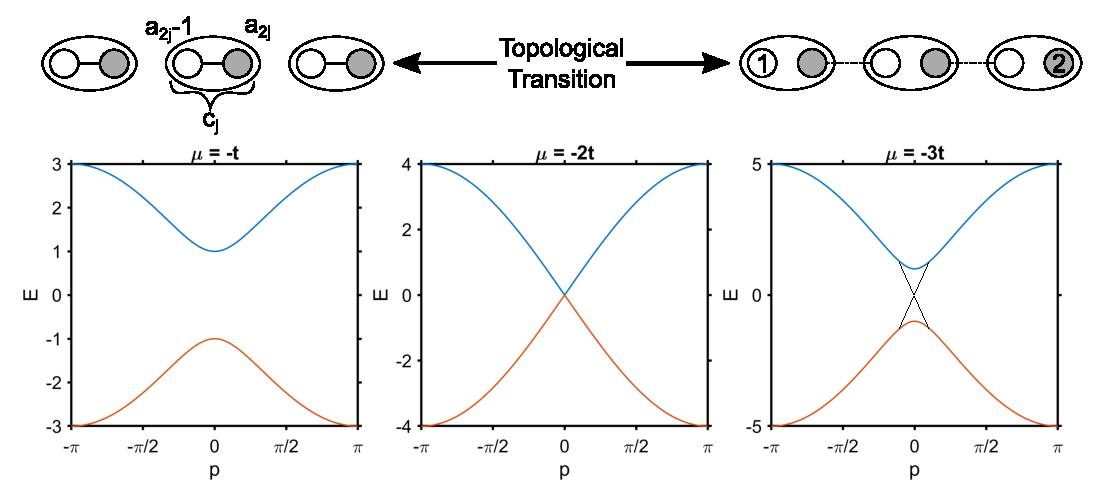
\includegraphics[width=\textwidth]{Intro/Figures/PWave_SC.eps}
	\caption{Dispersion relations of a 1D p-wave superconductor plotted at three different $\mu$ values. a) The trivial p-wave pairing scenario. The individual majorana particles each couple to the majorana on the same site. b) The critical value for $\mu$ where the gap closes. c) The topological p-wave pairing scenario. The majorana particles pair with majoranas on the nearest-neighbor site instead of on the same site. Two majorana zero modes are left on the edges of the wire, consistent with the bulk-boundary correspondence.}
	\label{fig:pwavesc}
\end{figure}
For an intuitive picture for why this is we will split the complex fermion operators into their Majorana fermion constituents. We replace each complex fermion $c_{j}$ with two Majorana fermions, $a_{2j-1},a_{2j}$ via $c_{j}=\frac{1}{2}(a_{2j-1}+ia_{2j})$ and $c_{j}^{\dagger}=\frac{1}{2}(a_{2j-1}-ia_{2j})$. The Majorana operators are fermionic and are defined by their property $a_{j}=a_{j}^{\dagger}$ therefore they satisfy $\{a_{j}^{\dagger},a_{j'}\}=2\delta_{jj'}$ as well as $\{a_{j},a_{j'}\}=2\delta_{jj'}$. As an aside, due to the latter relation we can always break up a complex fermion operator into its real and imaginary Majorana components, although it may not always be a useful representation. Now, the Hamiltonian for the lattice p-wave superconductor can be written as:
\begin{align}
	H_{BdG} = \frac{i}{2}\sum_{p}\left(-\mu a_{2j-1}a_{2j}+(t+|\Delta|)a_{2j}a_{2j+1}+(-t+|\Delta|)a_{2j-1}a_{2j+2}\right)
\end{align}
Here we can examine the difference between the two cases presented above by looking at two special limits.\par 
The first limit is the trivial phase when we choose $\mu < 0$ and $|\Delta|=t=0$. Here, the Hamiltonian reduces to,
\begin{align}
	H = -\mu\frac{i}{2}\sum_{j}(a_{2j-1}a_{2j})
\end{align}
In this phase, the Majorana operators on each site are coupled together with an energy $\mu/2$ but there is no coupling between Majorana operators on different sites (see Fig \ref{pwavesc}). This is denoted as the trivial phase since there will be no low-energy states on the end of the chain if the boundaries are cut between sites. Said another way, the Majorana operators are localized to each site and are therefore in the atomic limit which is to say the trivial ground state.\par 
The second limit is the topological phase where we choose $|\Delta|=t>0$ and $\mu=0$. Here, the Hamiltonian reduces to,
\begin{align}
	H=it\sum_{j}a_{2j}a_{2j+1}
\end{align}
This phase is the opposite of the previous phase as the Majorana operators on each site are only coupled to Majorana operators on \textit{different} sites with an energy $t$. When the chain is cut the Majorana operators $a_{1}$ and $a_{2L}$ ($L$ is the last site) are ``unpaired" and therefore there is a low-energy state on the each end of the chain (see Fig \ref{fig:pwavesc}). Comparing to before, it is impossible to adiabatically tune this phase back to the atomic limit without closing the bulk gap (see Fig \ref{fig:pwavesc}) and is thus a topologically non-trivial state. As a result, in the nontrivial phase the zero modes will not be destroyed until the bulk gap closes at a critical point.\par 
This last point, along with the self-adjoint property, make \ac{MZM} ideal candidates for fault-tolerant quantum computing. The self-adjoint property make \ac{MZM} a topological quantum object called an ``anyon", a quasi-particle that is in between a boson and fermion. Anyons braid non-trivially: two counterclockwise exchanges do not leave the state of the system invariant, unlike in the cases of bosons or fermions\cite{Sarma2015, Knapp2019}. In this manner, \ac{MZM} would be able to store information in the global wavefunction. That is to say the quantum state would be robust against local perturbations, drastically increasing the amount of quantum computations that could be made before the states decohere.\par 
While the model presented above provides an intuitive understanding of how \ac{MZM} arise out of the topological superconducting phase, there are no confirmed candidates for materials that would realize it. Fortunately, there are quite a few other proposed models of obtaining topological superconductivity and/or observing \ac{MZM} directly. These models include planar Josephson Junctions on a normal material that is subject to Rashba spin-orbit coupling\cite{Hell2017, Pientka2017, Whiticar2020}, \ac{MZM} arising as exotic excitations with fractional quantum numbers in Kitaev Quantum Spin Liquids\cite{KITAEV20062,Wang2020}, or inducing superconductivity into a topological insulator\cite{FuKane2008}. What is apparent is that to study some of these systems, new methods of fabrication must be made so that we can study a wider variety of candidate materials, including materials that are sensitive to water and oxygen. With this in mind, we go directly into the next chapter which discusses a brand new instrument that is able to fabricate, characterize, and measure devices without the materials ever seeing ambient air.